

 \documentclass[20pt, a0paper, portrait, margin=0mm, innermargin=15mm,
     blockverticalspace=15mm, colspace=15mm, subcolspace=8mm]{tikzposter} 

 \usepackage[utf8]{inputenc}
 \usepackage{tikz,multicol}
 \usepackage[absolute]{textpos}
 \usepackage{hyperref}
 \usepackage[caption=false]{subfig}
 \usepackage{xcolor,colortbl}
 \usepackage{float}
 \usepackage{amsmath}
 \usepackage{amsthm}
 \usepackage{amssymb}
 \usepackage{wrapfig}
 

 \newcommand{\bs}{\textbackslash}   % backslash
 \newcommand{\cmd}[1]{{\bf \color{red}#1}}   % highlights command

 % Title, Author, Institute
 \title{Briškula i umjetna inteligencija}
 \author{Ivan Laković \\ 
 {\fontfamily{qcr}\selectfont \Large
    \href{mailto:ilakovi@student.math.hr}{ilakovi@student.math.hr}}}
 \institute{PMF - Matematički odsjek}

 % Choose LAYOUT:  Default, Basic, Rays, Simple, Envelope, Wave, Board, Autumn, Desert,
 \usetheme{Wave}
\usecolorstyle[colorPalette=BrownBlueOrange]{Germany}
%\usecolorstyle[colorPalette=GreenGrayViolet]{Germany}
%\usecolorstyle[colorPalette=PurpleGrayBlue]{Denmark}
%\usecolorstyle[colorPalette=BlueGrayOrange]{Denmark}
%\usecolorstyle[colorPalette=BlueGrayOrange]{Sweden}
%\usecolorstyle[colorPalette=GrayOrangeBlue]{Denmark}
%\usecolorstyle[colorPalette=BlueGrayOrange]{Denmark}

\definecolor{orange}{RGB}{255,153,255}
\definecolor{blue1}{RGB}{204,0,255}
\definecolor{blue2}{RGB}{76,120,255}
\definecolor{blue3}{RGB}{120,88,243}
\definecolor{blue4}{RGB}{180,0,194}
\definecolor{blue5}{RGB}{76,150,215}
\definecolor{blue6}{RGB}{173,31,194}
\definecolor{blue7}{RGB}{255,71,143}
\definecolor{blue8}{RGB}{196,8,125}
\definecolor{blue9}{RGB}{180,56,215}
\definecolor{blue22}{RGB}{255,204,255}
\definecolor{blue23}{RGB}{232,153,227}
\definecolor{blue24}{RGB}{185,122,181}

\newtheorem*{teorem}{Teorem}
\newtheorem*{korolar}{Korolar}


 \begin{document}

    \maketitle

   

    \begin{columns}%blocks will be placed into columns
     
    \column{.55}
    
        \block[roundedcorners=40]{\color{blue1}O briškuli}{
            
            Briškula (Briscola) je talijanska kartaška igra udomaćena na hrvatskom priobalju i otocima.
            \begin{itemize}
                \item u špilu ima 40 karata.
                \item postoje 4 tipa po 10 karata: kope, baštone, špade i dinari
                \item nakon sto svi igrači bace kartu, rundu uzima igrač koji je bacio najjaču briškulu ili ako briškule nema, igrač koji je bacio najjaču kartu iste boje kao i igrač koji je igrao prvi u trenutnoj rundi.
            \end{itemize}
          
        }
        \begin{subcolumns}
        \subcolumn{.39}
        \block{\color{blue24}Primjer stabla}{
            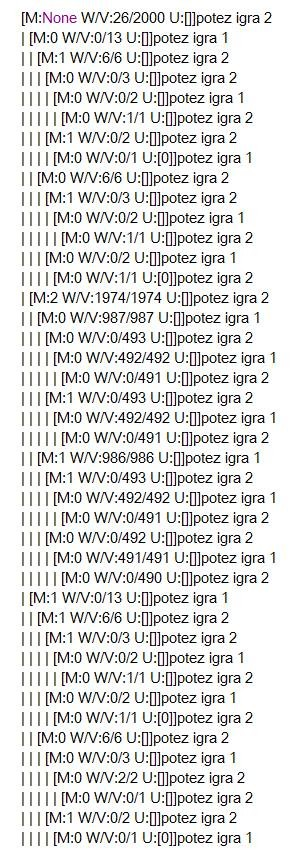
\includegraphics[width=0.10\textwidth]{uct_stablo}
            \vskip1ex
            Stablo pretraživanja UCT-a \colorbox{blue22}{3 koraka prije kraja igre}. \newline Vidi se da ako odigra kartu s rednim brojem 2 sigurno pobjeđuje, te je to i razlog zašto bacanje te karte češće analizira u odnosu na druge dvije. \newline Iz ovakvog stabla vidljivo je koju kartu će UCT odigrati i zašto.
        }
        \note[rotate=90, targetoffsetx=-65pt]{Kako UI vidi poteze}
        
        
        \block{}{
            \begin{tikzfigure}[Podijeljene karte]
                \centering
               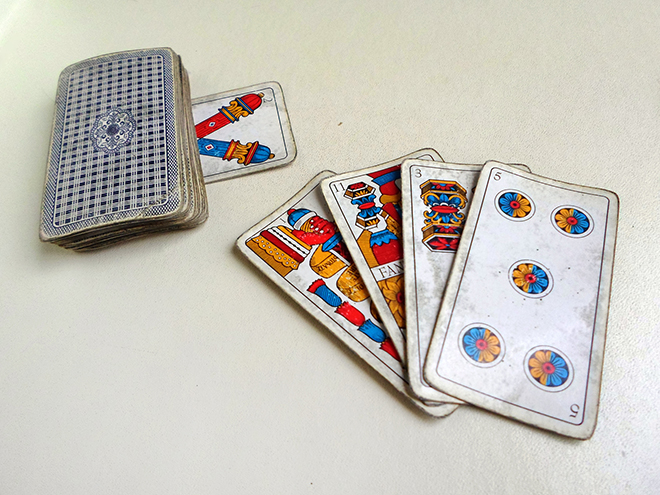
\includegraphics[width=0.15\textwidth, angle=90]{briskula_spil}
            \end{tikzfigure}
            Kad igra započne svakom igraču se dijeli 3/4 karte te se jedna okrene licem prema gore, te ona označava briškulu.
        }
        
        \subcolumn{.61}
        \block{\color{blue3}Monte Carlo stablo pretraživanja}{
            Monte Carlo stablo pretraživanja je heuristički algoritam pretraživanja koji se koristi u procesima donošenja odluka, najčešće u igranju igara. Samom algoritmu prethodio je John von Neumannov teorem.
            \begin{teorem}{Minimax teorem}
                Neka su $ X \subset \mathbb{R}^n $ i $ Y \subset \mathbb{R}^m $ kompaktni konveksni skupovi. Ako je $ f : X \times Y \rightarrow \mathbb{R} $ neprekidna funkcija koja je konveksno-konkavna. Tada slijedi:
                \begin{equation}
                    \label{jed:1}
                    \min_{x \in X} \max_{y \in Y} f(x,y) = \max_{y \in Y} \min_{x \in X} f(x,y)
                \end{equation}
            \end{teorem}
            Minimax teorem \eqref{jed:1} formirao je bazu za teoriju odlučivanja u računarstvu i AI-u. Algoritam simulira igru zadani broj puta te pronalazi optimalan potez. Svaka simulacija igre se sastoji od iduća 4 koraka:
            \begin{enumerate}
                \item \colorbox{blue22}{Odabir} - odabir najuspješnijega djeteta.
                \item \colorbox{blue22}{Proširivanje} - ako nije kraj igre odigra potez.
                \item \colorbox{blue22}{Simulacija} - odigra simulaciju do kraja.
                \item \colorbox{blue22}{Ažuriranje znanja} - ažurira odigrani potez ovisno o rezultatu.
            \end{enumerate}
            
            \vskip2ex
            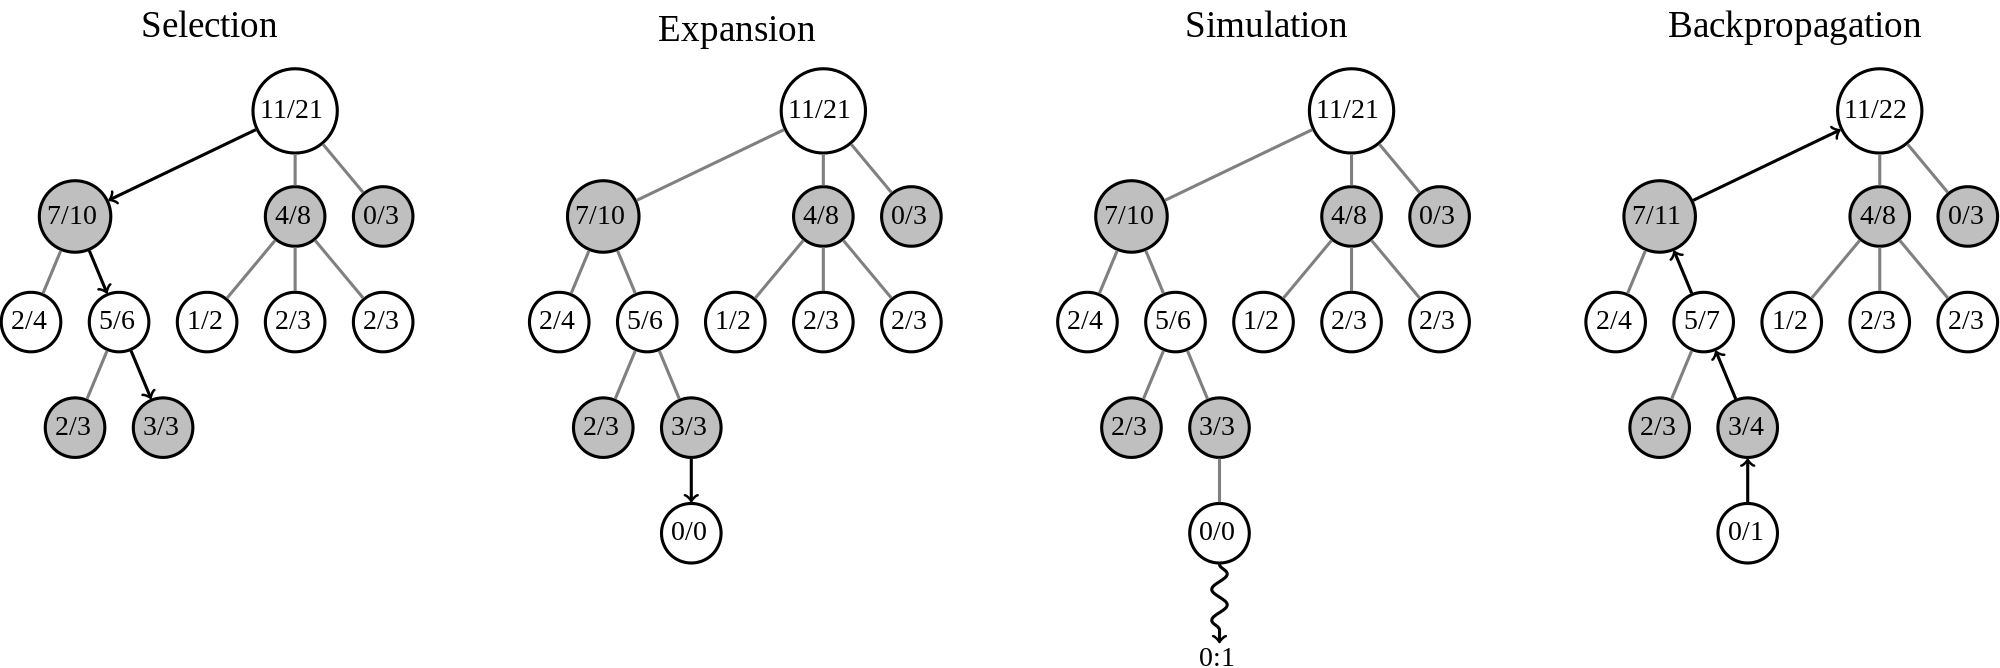
\includegraphics[width=0.3\textwidth]{MCTS}
            \vskip2ex
        }
        
        \block{\color{blue4}UCT algoritam}{
           Najteži posao je održati ravnotežu između iskorištavanja kombinacija koje donosi odabir djeteta s visokim stupnjem pobjeda i proširivanja poteza s malim brojem simulacija. Prva uspješna formula koja je to ostvarila je UCB:
           \begin{equation} 
               \label{jed:2} 
               \frac{w_i}{n_i} + c * \sqrt{\frac{\ln{t}}{n_i}} \qquad
           \end{equation} 
                  gdje je:
            \begin{itemize}
                \item $w_i$ označava broj pobjeda nakon i-tog poteza
                \item $n_i$ označava broj simulacija nakon i-tog poteza
                \item c je parametar iskorištavanja, teoretski je uvijek $\sqrt{2}$
                \item t označava ukupan broj simulacija koji odgovara sumi $n_i$-ova
            \end{itemize}
            Prvi dio formule \eqref{jed:2} zadužen je za produbljivanje postojećeg stanja, a drugi za proširivanje stabla radi problema lokalnog ekstrema. \newline Dokazano je da procjena najboljih poteza u MCTS algoritmu konvergira minimax procjeni. \newline
            UCT je poseban slučaj MCTS algoritma te se može opisati kao:
            \begin{equation}
                UCT = MCTS + UCB
            \end{equation}

        }
        
        \end{subcolumns}
        
        \block[titlewidthscale=.95,bodywidthscale=.9,titleoffsety=9.5mm,bodyoffsety=9mm]{\color{blue23}Zaključak}{
            U testiranju algoritma protiv čovjeka, algoritam igra vrlo dobro, te u većini slučajeva pobjedi. Prednosti alogritma su:
            \begin{itemize}
                \item ne zahtjeva nikakve heuristike 
                \item daje dobre rezultate već pri malom broju simulacija
            \end{itemize}
            Osnovni algoritam može se poboljšati tako da osim nastojanja u tome da pobjedi pokuša i maksimizirati konačan broj bodova. Osim toga, mogla bi se uvesti i heuristika koja će mu ograničiti broj karti koje je dopušteno baciti. U slučaju dobre heuristike, smanjilo bi se grananje stabla, i ubrzalo računanje. \newline
            U proučavanju igranja algoritma nismo uočili nikakvu nama razumljivu heuristiku kod izbora karte za bacanje stoga smo zaključili da je svaki potez specijalan te se igranje poput algoritma ne može naučiti. 
        }
        

    \column{.45}
        \block{\color{blue6}Sažetak}{
        
            Cilj projekta je bio dokazati da će se umjetna inteligencija moći nositi s ljudskim igračima u igri briškula za koju se smatra da najvećim dijelom čista sreća, a manjim dijelom znanje i taktika. \newline 
            U slučaju da je umjetna inteligencija bolja od ljudskog igrača želja nam je bila vidjeti razliku u načinu igre, te pokušati i sami naučiti igrati na taj bolji način. \newline
            Umjetnu inteligenciju odlučili smo implementirati pomoću algoritma \colorbox{blue22}{Monte Carlo tree search}. \newline
            Važan čimbenik u odabiru je bila i nedavna pobjeda Google-ovog AI-a \colorbox{blue22}{AlphaGo} u igri Go (posljednja igra na ploči u kojoj je čovjek mogao pobijediti računalo) umjetna inteligencija koristila kombinaciju dubokog učenja i MCTS algoritma.
        
        }

         \begin{subcolumns}
            \subcolumn{.05}
            \subcolumn{.49}
            \block{\color{blue7}UCT vs UCT}{
                Borba umjetnih inteligencija s različitim brojem simulacija igre po potezu.
                U tablici je prosječan
                \vskip2ex
                \begin{center}
                
                    \begin{tabular}{||c c c||} 
                        \hline
                        \rowcolor{blue1}
                        UCT 1 & UCT 2 & Omjer pobijeda \\ [0.5ex] 
                        \hline\hline
                        \rowcolor{blue23}
                        300 & 500 & 25:25\\ 
                        \hline
                        \rowcolor{blue22}
                        500 & 750 & 26:24\\
                        \hline
                        \rowcolor{blue23}
                        300 & 1000 & 15:35\\
                        \hline
                        \rowcolor{blue22}
                        500 & 1000 & 21:29\\
                        \hline
                        \rowcolor{blue23}
                        800 & 1000 & 19:31\\
                        \hline
                        \rowcolor{blue22}
                        900 & 1000 & 27:23\\
                        \hline
                        \rowcolor{blue23}
                        1000 & 1500 & 25:25\\
                        \hline
                        \rowcolor{blue22}
                        300 & 2000 & 16:34\\
                        \hline
                        \rowcolor{blue23}
                        500 & 2000 & 22:28\\
                        \hline
                        \rowcolor{blue22}
                        750 & 2000 & 22:28\\
                        \hline
                        \rowcolor{blue23}
                        1000 & 2000 & 22:28\\
                        \hline
                        \rowcolor{blue22}
                        1500 & 2000 & 23:27\\
                        \hline
                        \rowcolor{blue23}
                        1750 & 2000 & 22:28\\
                        \hline
                        \rowcolor{blue22}
                        2000 & 2500 & 23:27\\
                        \hline
                        \rowcolor{blue23}
                        2000 & 3000 & 26:24\\
                        \hline
                        \rowcolor{blue22}
                        2000 & 4000 & 27:23\\
                        \hline
                        \rowcolor{blue23}
                        500 & 5000 & 22:28\\
                        \hline
                        \rowcolor{blue22}
                        2000 & 5000 & 27:23\\
                        \hline
                        \rowcolor{blue23}
                        2000 & 10000 & 24:26\\ [1ex] 
                        \hline
                    \end{tabular}
                \end{center}
                \vskip2ex
                Iz tablice je vidljivo da je optimalan broj simulacija oko 2000.

             
             }

             \subcolumn{.46}
             \block{\color{blue8}Važni pojmovi}{
                \begin{itemize}
                    \item MCTS - Monte Carlo Tree Search, algoritam za korištenje stabla pretraživanja
                    \item UCT - Upper Confidence Bound 1 applied to trees, implementacija MCTS koja balansira proširivanje i produbljivanje stabla pretraživanja
                    \item Stablo pretraživanja - stablo u kojem svaki čvor sadrži podatke o broju pobjeda u odnosu na broj simulacija za svaki odigrani potez 
                    \item Briškula - kartaška igra, popularna u priobalju Jadranskog mora, ujedno i naziv boje koja trenutno vodi igru
                    \item AlphaGo - Googleov program, prvi program koji je pobijedio ljudskog protivnika u igri Go  
                \end{itemize}
                
             }
        \end{subcolumns}


        \block[titlewidthscale=.95,bodywidthscale=.9,titleoffsety=9.5mm,bodyoffsety=9mm]{\color{blue9} Testiranje algoritma}{
            Algoritam smo osim igranjem protiv njega, radi lakšeg i bržeg testiranja odlučili testirati na 3 načina:
            \begin{enumerate}
                \item Borbom protiv samog sebe s različitim brojem iteracija.
                \item Borbom protiv heuristike koja simulira igranje čovjeka
                \item Borbom protiv samog sebe s različitim koeficijentom c u UCT formuli.
            \end{enumerate}
            
            \begin{enumerate}
                \item U borbi protiv samog sebe pokušali smo pronaći optimalan broj iteracija tako da se na
odgovor algoritma ne čeka previše, ali opet da bude dobro obaviješten. Kao što se vidi iz tablice, optimalan broj iteracija je oko 2000. Ako mu suprotstavimo UCT s manjim brojem iteracija primjećujemo da UCT s 2000 iteracija uvijek pobijedi više od 50\% puta, dok u suprotnom slučaju kad se bori protiv UCT-a s više iteracija rezultat nije predvidljiv.

                \item U borbi protiv naše heuristike igra završi gotovo
uvijek jednako, to jest UCT uvijek prevlada, ali bez obzira na broj iteracija, kako briškula ipak ima
udio sreće nikad ne uspije pobijediti u 100\% slučajeva.

                \item Borbom UCT-a s istim brojem iteracija, a različitim koeficijentima pri čemu jedan UCT ima
fiksiran koeficijent od $\sqrt(2)$ zaključujemo da veličina izabranoga koeficijenta c ukoliko je on u intervalu
između 0.4 i 20 ne mijenja bitno situaciju, te zbog nausumičnosti podjele karata broj pobjeda varira.
            \end{enumerate}


        }
        
        
        \block[titlewidthscale=.95,bodywidthscale=.9,titleoffsety=9.5mm,bodyoffsety=9mm]{\color{blue9}Link na igricu}{
            
            \vspace{-2ex} 
                Za pokrenuti igru treba: skinuti i raspakirati mapu s danog linka. Na izboru su 4 opcije igranja: easy, medium, hard te igranje s otovorenim kartama.

                \begin{tikzfigure}[QRcode]
                   \centering
                   
\includegraphics[width=0.1\textwidth]{qrcode}
                \end{tikzfigure}
        }
        \note[rotate=30, targetoffsetx=1pt]{https://goo.gl/a2bMXZ}
        
        
        
        
    \end{columns}



    
\end{document}




\endinput
%%
%% End of file `tikzposter-example.tex'.
